\chapter{Mining Class-Specific Alterations in Binary Data}\label{chap:CSalt}
When given labeled data, a natural instinct for a data miner is to build a discriminative model that predicts the correct class.
Yet in this chapter we focus on the characterization of the data with respect to the label in order to find similarities and differences between chunks of data belonging to miscellaneous classes.
Consider a binary matrix where each row is assigned to one class. Such data emerge from fields such as gene expression analysis, e.g., a row reflects the genetic information of a cell, assigned to one tissue type (primary/relapse/no tumor), market basket analysis, e.g., a row indicates purchased items at the assigned store, or from text analyses, e.g., a row corresponds to a document/article and the class denotes the publishing platform. For various applications a characterization of the data with respect to classes is of particular interest. In genetics, filtering the genes which are responsible for the reoccurrence of a tumor may introduce new possibilities for personalized medicine~\citep{schramm2015mutational}. In market basket analysis it might be of interest which items sell better in some shops  than others and in text analysis one might ask about variations in the vocabulary used when reporting from diverse viewpoints.
%--------- FIGURE FACTORIZE EACH CLASS SEPARATELY ------------
 \begin{figure}
 \centering
 {%\tiny
$
\begin{tikzpicture}[decoration=brace,baseline=-0.5ex]
   \matrix [matrix of math nodes,left delimiter=(,right delimiter=)] (n) {
1&1&1&\textcolor{red}{1}&1&1&0&0&0\\
0&0&1&0&1&1&0&0&0\\
1&1&0&\textcolor{red}{1}&0&1&0&0&0\\
1&1&1&\textcolor{red}{1}&1&1&0&0&0\\
0&0&0&0&0&0&1&1&0\\
1&1&0&0&0&1&1&1&\textcolor{red}{1}\\
1&1&0&0&0&1&0&0&\textcolor{red}{1}\\
0&0&0&0&0&0&1&1&0\\
};
%-- brackets ----
\draw[decorate,transform canvas={xshift=-1.5em}] (n-4-1.south west) -- node[left=2pt] {$A$} (n-1-1.north west);
\draw[decorate,transform canvas={xshift=-1.5em}] (n-8-1.south west) -- node[left=2pt] {$B$} (n-5-1.north west);
%--- blue ---
\draw[color=col1,fill=col1,opacity=0.3] (n-1-5.north west) -- (n-1-6.north east) -- (n-2-6.south east) -- (n-2-5.south west) -- (n-1-5.north west);
\draw[color=col1,fill=col1,opacity=0.3] (n-4-5.north west) -- (n-4-6.north east) -- (n-4-6.south east) -- (n-4-5.south west) -- (n-4-5.north west);
\draw[color=col1,fill=col1,opacity=0.3] (n-1-3.north west) -- (n-1-3.north east) -- (n-2-3.south east) -- (n-2-3.south west) -- (n-1-3.north west);
\draw[color=col1,fill=col1,opacity=0.3] (n-4-3.north west) -- (n-4-3.north east) -- (n-4-3.south east) -- (n-4-3.south west) -- (n-4-3.north west);
%--- green ---
\draw[color=col2,fill=col2,opacity=0.3] (n-5-7.north west) -- (n-5-8.north east) -- (n-6-8.south east) -- (n-6-7.south west) -- (n-5-7.north west);
\draw[color=col2,fill=col2,opacity=0.3] (n-8-7.north west) -- (n-8-8.north east) -- (n-8-8.south east) -- (n-8-7.south west) -- (n-8-7.north west);
\draw[color=col1,fill=col1,opacity=0.3] (n-1-3.north west) -- (n-1-3.north east) -- (n-2-3.south east) -- (n-2-3.south west) -- (n-1-3.north west);
\draw[color=col1,fill=col1,opacity=0.3] (n-4-3.north west) -- (n-4-3.north east) -- (n-4-3.south east) -- (n-4-3.south west) -- (n-4-3.north west);
%-- pink ---
\draw[color=col3,fill=col3,opacity=0.3] (n-1-1.north west) -- (n-1-2.north east) -- (n-1-2.south east) -- (n-1-1.south west) --(n-1-1.north west);
\draw[color=col3,fill=col3,opacity=0.3] (n-1-6.north west) -- (n-1-6.north east) -- (n-1-6.south east) -- (n-1-6.south west) --(n-1-6.north west);
\draw[color=col3,fill=col3,opacity=0.3] (n-3-1.north west) -- (n-3-2.north east) -- (n-4-2.south east) -- (n-4-1.south west) --(n-3-1.north west);
\draw[color=col3,fill=col3,opacity=0.3] (n-3-6.north west) -- (n-3-6.north east) -- (n-4-6.south east) -- (n-4-6.south west) --(n-3-6.north west);
\draw[color=col3,fill=col3,opacity=0.3] (n-6-1.north west) -- (n-6-2.north east) -- (n-7-2.south east) -- (n-7-1.south west) --(n-6-1.north west);
\draw[color=col3,fill=col3,opacity=0.3] (n-6-6.north west) -- (n-6-6.north east) -- (n-7-6.south east) -- (n-7-6.south west) --(n-6-6.north west);
\end{tikzpicture}
\approx
\begin{tikzpicture}[baseline=-0.5ex]
    \matrix [matrix of math nodes,left delimiter=(,right delimiter=)] (n) {
1&1&0 \\
0&1&0 \\
1&0&0 \\
1&1&0 \\
0&0&1 \\
1&0&1 \\
1&0&0\\
0&0&1 \\
};
%---- blue ---
\draw[color=col1,fill=col1,opacity=0.3] (n-1-2.north west) -- (n-1-2.north east) -- (n-2-2.south east) -- (n-2-2.south west) -- (n-1-2.north west);
\draw[color=col1,fill=col1,opacity=0.3] (n-4-2.north west) -- (n-4-2.north east) -- (n-4-2.south east) -- (n-4-2.south west) -- (n-4-2.north west);
%---- green ---
\draw[color=col2,fill=col2,opacity=0.3] (n-5-3.north west) -- (n-5-3.north east) -- (n-6-3.south east) -- (n-6-3.south west) -- (n-5-3.north west);
\draw[color=col2,fill=col2,opacity=0.3] (n-8-3.north west) -- (n-8-3.north east) -- (n-8-3.south east) -- (n-8-3.south west) -- (n-8-3.north west);
%--- pink ---
\draw[color=col3,fill=col3,opacity=0.3] (n-1-1.north west) -- (n-1-1.north east) -- (n-1-1.south east) -- (n-1-1.south west) --(n-1-1.north west);
\draw[color=col3,fill=col3,opacity=0.3] (n-3-1.north west) -- (n-3-1.north east) -- (n-4-1.south east) -- (n-4-1.south west) --(n-3-1.north west);
\draw[color=col3,fill=col3,opacity=0.3] (n-6-1.north west) -- (n-6-1.north east) -- (n-7-1.south east) -- (n-7-1.south west) --(n-6-1.north west);
\end{tikzpicture}
\cdot
\begin{tikzpicture}[baseline=-0.5ex]
    \matrix [matrix of math nodes,left delimiter=(,right delimiter=)] (n) {
1&1&0&0&0&1&0&0&0 \\
0&0&1&0&1&1&0&0&0 \\
0&0&0&0&0&0&1&1&0 \\
};
%--- blue ---
\draw[color=col1,fill=col1,opacity=0.3] (n-2-3.north west) -- (n-2-3.north east) -- (n-2-3.south east) -- (n-2-3.south west) -- (n-2-3.north west);
\draw[color=col1,fill=col1,opacity=0.3] (n-2-5.north west) -- (n-2-6.north east) -- (n-2-6.south east) -- (n-2-5.south west) -- (n-2-5.north west);
%--- green ---
\draw[color=col2,fill=col2,opacity=0.3] (n-3-7.north west) -- (n-3-8.north east) -- (n-3-8.south east) -- (n-3-7.south west) -- (n-3-7.north west);
%---- pink ---
\draw[color=col3,fill=col3,opacity=0.3] (n-1-1.north west) -- (n-1-2.north east) -- (n-1-2.south east) -- (n-1-1.south west) --(n-1-1.north west);
\draw[color=col3,fill=col3,opacity=0.3] (n-1-6.north west) -- (n-1-6.north east) -- (n-1-6.south east) -- (n-1-6.south west) --(n-1-6.north west);
\end{tikzpicture}
$
}

 \caption{A Boolean factorization of rank three. The data matrix on the left is composed by transactions belonging to two classes $A$ and $B$. Each outer product is highlighted. Best viewed in color.}
 \label{fig:classFact}
 \end{figure}
%-------------------------------------

These questions are approached as pattern mining~\citep{vreeken2007characterising} and Boolean matrix factorization problems~\citep{miettienen2012finding}. Both approaches search for factors or patterns which occur in both or only one of the classes. This is illustrated in Figure~\ref{fig:classFact}; a data matrix is indicated on the left, whose rows are assigned to one class, $A$ or $B$. While the green outer product spreads over both classes, the blue products concentrate in only one of the classes. We refer to the factorizations of the first kind as common and to those of the second kind as class-specific.

The identification of class specific and common factorizations is key to a characterization of similarities and differences among the classes. Yet, what if meaningful deviations between the classes are slightly hidden underneath an overarching structure? The factorization in Figure~\ref{fig:classFact} is not exact, we can see that the red colored ones in the data matrix are not taken into account by the model (the factorization on the right). This is partially desired as the data is expected to contain noise which is supposedly filtered out. On the other hand, we can observe concurrence of the red ones and the pattern of the green tile -- in each class.
%------------------------
% Main Contributions
%------------------------
%\subsection{Main Contributions}
In this chapter we propose a novel Boolean matrix factorization method which is suitable to compare horizontally concatenated binary data matrices originating from diverse sources or belonging to various classes. To the best of the authors knowledge, this is the first method in the field of matrix factorizations of any kind, combining the properties listed below in one framework:
\begin{itemize}
\item the method can be applied to compare any number of classes or sources,
\item the factorization rank is automatically determined; this includes the automatic identification of tiles being common among multiple classes as well as the identification of discriminative tiles occurring in only one class,
\item in addition to discriminative tiles, more subtle characteristics of classes can be derived, pointing out the features where common tiles deviate among the classes.
\end{itemize}
While works exist which approach one of the first two  points mentioned above (cf.\@ Section~\ref{sec:CS:IntegrateLabels}), the focus on subtle deviations among the classes as addressed in the third point is entirely new. This expands the applicability of the new method to datasets where deviations among the classes have a more complex structure.
%========================
% integrating class labels into BMF
%========================
\section{Integrating Class Labels and BMF}\label{sec:CS:IntegrateLabels}
We assume that the data matrix is composed of various sources, represented by an assignment of transactions to $c$ classes. Denoting by $[A^{(a)}]_a$ the matrix vertically concatenating the matrices $A^{(a)}$ for $a\in\{1,\ldots,c\}$, that is the matrices are stacked on top of each other, we write
\begin{align}\label{eq:CS:DaYaVa}
D=\begin{bmatrix}
D^{(a)}
\end{bmatrix}_a,\
Y=\begin{bmatrix}
Y^{(a)}
\end{bmatrix}_a \text{ and }
V^\top =\begin{bmatrix}
V^{(a)T}
\end{bmatrix}_a.
\end{align}
The $m_a\times n$ matrix $D^{(a)}$ comprises the $m_a$ transactions belonging to class $a$. The total number of transactions is therefore given by $m=m_1+\ldots+m_c$. Likewise, we explicitly notate the class-related $m_a\times r$- and $n\times r$-dimensional parts of the $m\times r$ and $n\times rc$ factor matrices $Y$ and $V$ as $Y^{(a)}$ and $\Va$. These factor matrices are properly introduced in Section~\ref{sec:CS:CSalt}.
%--------- FIGURE USAGE ------------
\begin{figure}[!t]
\centering
{%\tiny
$
\begin{tikzpicture}[decoration=brace,baseline=-0.5ex]
   \matrix [matrix of math nodes,left delimiter=(,right delimiter=), every node/.append style={text width=0.3cm,align=center,minimum width=4ex, minimum height=3.5ex},
  nodes in empty cells,] (n) {
&&&&\\
&&&&\\
&&&&\\
&&&&\\
&&&&\\
&&&&\\
};
%--- matrix names---
\node[font=\normalsize] 
  at ([xshift=-1pt, yshift=-3pt]n-3-1) {$Y_{S}$};
\node[font=\normalsize] 
  at ([xshift=-5pt, yshift=-2pt]n-2-3) {$Y^{(1)}_{D}$};
  \node[font=\normalsize] 
  at ([xshift=-5pt, yshift=-2pt]n-5-5) {$Y^{(2)}_{D}$};
%== brackets ==
%-- m_1,m_2 ------
\draw[decorate,transform canvas={xshift=-1.5em}] (n-3-1.south west) -- node[left=2pt] {$m_1$} (n-1-1.north west);
\draw[decorate,transform canvas={xshift=-1.5em}] (n-6-1.south west) -- node[left=2pt] {$m_2$} (n-4-1.north west);
%-- ranks ---
\draw[decorate,transform canvas={yshift=-1em}] (n-6-1.south east) -- node[below=2pt] {$r_0$} (n-6-1.south west);
\draw[decorate,transform canvas={yshift=-1em}] (n-6-3.south east) -- node[below=2pt] {$r_1$} (n-6-2.south west);
\draw[decorate,transform canvas={yshift=-1em}] (n-6-5.south east) -- node[below=2pt] {$r_2$} (n-6-4.south west);
%=== colors ===
%--- blue ---
\draw[color=col1,fill=col1,opacity=0.3] (n-1-2.north west) -- (n-1-3.north east) -- (n-3-3.south east) -- (n-3-2.south west) -- (n-1-2.north west);
%--- green ---
\draw[color=col2,fill=col2,opacity=0.3] (n-4-4.north west) -- (n-4-5.north east) -- (n-6-5.south east) -- (n-6-4.south west) -- (n-4-4.north west);
%-- pink ---
\draw[color=col3,fill=col3,opacity=0.3] (n-1-1.north west) -- (n-1-1.north east) -- (n-6-1.south east) -- (n-6-1.south west) --(n-1-1.north west);
\end{tikzpicture}
%------------- X-------------------
\qquad\odot
\begin{tikzpicture}[decoration=brace,baseline=-0.5ex]
   \matrix [matrix of math nodes,left delimiter=(,right delimiter=), every node/.append style={text width=0.2cm,align=center,minimum height=3ex},
  nodes in empty cells,] (n) {
&&&&&&\\
&&&&&&\\
&&&&&&\\
&&&&&&\\
&&&&&&\\
};
%--- matrix names---
\node[font=\normalsize] 
  at (n-1-4) {$X_{S}^T$};
\node[font=\normalsize] 
  at ([yshift=-6pt]n-2-4) {$X_1^T$};
  \node[font=\normalsize] 
  at ([yshift=-6pt]n-4-4) {$X_2^T$};
%== brackets ==
%-- m_1,m_2 ------
\draw[decorate,transform canvas={xshift=-1.5em}] (n-1-1.south west) -- node[left=2pt] {$r_0$} (n-1-1.north west);
\draw[decorate,transform canvas={xshift=-1.5em}] (n-3-1.south west) -- node[left=2pt] {$r_1$} (n-2-1.north west);
\draw[decorate,transform canvas={xshift=-1.5em}] (n-5-1.south west) -- node[left=2pt] {$r_2$} (n-4-1.north west);
%-- ranks ---
\draw[decorate,transform canvas={yshift=-1em}] (n-5-7.south east) -- node[below=2pt] {$n$} (n-5-1.south west);
%=== colors ===
%--- blue ---
\draw[color=col1,fill=col1,opacity=0.3] (n-2-1.north west) -- (n-2-7.north east) -- (n-3-7.south east) -- (n-3-1.south west) -- (n-2-1.north west);
%--- green ---
\draw[color=col2,fill=col2,opacity=0.3] (n-4-1.north west) -- (n-4-7.north east) -- (n-5-7.south east) -- (n-5-1.south west) -- (n-4-1.north west);
%-- pink ---
\draw[color=col3,fill=col3,opacity=0.3] (n-1-1.north west) -- (n-1-7.north east) -- (n-1-7.south east) -- (n-1-1.south west) --(n-1-1.north west);
\end{tikzpicture}
$
}
\caption{A Boolean product identifying common (green) and class-specific outer products (blue). Best viewed in color.}
\label{fig:CS:usageJSMF}
\end{figure}
%-------------------------------------
If the given data matrix is classwise concatenated (cf.\@ Eq.~(\ref{eq:CS:DaYaVa})), a first approach for finding class-defining characteristics is to separately derive factorizations for each class. However, simple approximation measurements such as the residual sum of squares of a Boolean factorization are already nonconvex and have multiple local optima.
Due to this local view of computed models, classwise factorizations are not easy to interpret; they lack a view on the global structure. Puzzling together the (parts of) patterns defining (dis-)similarities of classes afterwards, is not trivial.

In the case of nonnegative, labeled data matrices, measures such as Fisher's linear discriminant criterion are minimized to derive weighted feature vectors, that are patterns in the binary case, which discriminate most between classes. This variant of NMF is successfully implemented for classification problems such as face recognition~\citep{nikitidis2014projected} and identification of cancer-associated genes~\citep{odibat2014efficient}.

For social media retrieval, \cite{gupta2010nonnegative} introduce Joint Subspace Matrix Factorization (JSMF). Focusing on the two-class setting, they assume that data points emerge not only from discriminative but also from common subspaces. JSMF infers for a given nonnegative data matrix and ranks $r_0,r_1$ and $r_2$ a factorization as displayed in Figure~\ref{fig:CS:usageJSMF}. Note that there are exactly $r_0$ columns in the factor matrix $Y$ spanning over points from both classes and $r_1$ respectively $r_2$ columns whose nonzero entries are restricted to class one or two. Multiplicative updates are used to minimize a weighted sum of classwise computed residual sums of squares.
%\[\min_{X,Y}\sum_{a\in\{1,2\}}\frac{\mu_a}{2}\left\|\Da-\begin{bmatrix}
%\Ya_S & \Ya_D
%\end{bmatrix} \begin{bmatrix}
%	X_S^\top \\
%    X_a^\top 
%\end{bmatrix}^\top \right\|^2,\]
%where $\mu_1^{-1} =\|D^{(1)}\|^2$ and $\mu_2^{-1} =\|D^{(2)}\|^2$ are normalizing constants.
In Regularized JSNMF (RJSNMF), a regularization term is used to prevent that shared feature vectors (in $X_S^\top $) swap into discriminative subspaces and vice versa~\citep{gupta2013regularized}. This happens if a column in $Y_S$ is divided into two columns, one in $Y_D^{(1)}$ and the other in $Y_D^{(2)}$. Correspondingly, a discriminative feature vector in $X_{1/2}$ could be represented as one of the shared vectors. The arising optimization problem is solved by the method of Lagrange multipliers. Furthermore, a provisional method to determine the rank automatically is evaluated. However, this involves multiple runs of the algorithm with increasing numbers of shared and discriminative subspaces, until the approximation error barely decreases.
A pioneering extension to the multi-class case  is provided by~\cite{gupta2014matrix}.

\cite{miettienen2012finding} transfers the objective of JSMF into Boolean algebra, solving
\[\min_{X,Y}\sum_{a\in\{1,2\}}\frac{\mu_a}{2}\left|\Da-\theta\left(\begin{bmatrix}
\Ya_{S} & \Ya_D
\end{bmatrix} \begin{bmatrix}
	X_S^\top \\
    X_a^\top 
\end{bmatrix}\right)\right|\]
for binary matrices $D, X$ and $Y$, and normalizing constants $\mu_{1/2}^{-1} =|D^{(2)/(1)}|$.  A variant of the BMF algorithm \textsc{Asso} governs the minimization. A provisional determination of ranks based on the MDL principle is proposed, computing which of the candidate rank constellations yields the lowest description length.

\cite{vreeken2007characterising} pursue the idea of MDL in the context of deriving a set of pattern sets, which characterizes similarities and differences of groups of classes. Identifying the usage of each pattern with its support in the data, the number of derived patterns equates the rank in BMF. In this respect, their proposed algorithm \textsc{DiffNorm} automatically determines the ranks in the multi-class case. However, as known from pattern mining, restricting the usage to the supporting transactions often results in a vast amount of returned patterns.    

In the case where two-classes are given for a nonnegative data matrix, \cite{kim2015simultaneous} improve over RJSNMF by allowing small deviations from shared patterns in each class. They found that shared patterns are often marginally altered according to the class. In this work, we aim at finding these overlooked variations of shared patterns together with strident differences among multiple classes, combining the strengths of MDL for rank detection and the latest results in NMF.
%===================================
%Mining class-specific alterations
%====================================
\section{Mining Class-Specific Alterations}
Given a binary data matrix composed from multiple classes, we assume that the data has an underlying model similar to the one in Figure~\ref{fig:classFact}. There are common or shared patterns (green) and class-specific patterns (blue). Furthermore, there are class-specific patterns, which align within a subset of the classes where a pattern is used (the red ones). We call such aligning patterns class-specific alterations and introduce the matrix $V$ to reflect them.
%-----------------------
\begin{definition}[class-specific alterations]\label{def:CS:classSpecAlt}
Let $X\in\{0,1\}^{n\times r}$ and $V\in \{0,1\}^{n\times cr}$ be binary matrices.
We say the matrix $V$ models \emph{class-specific alterations of $X$} if $\|X\circ \Va\|=0$ for all $1\leq a\leq c$, and $\|V^{(1)}\circ\ldots\circ V^{(c)}\|=0$.
\end{definition}
We assume that the data emerges from a Boolean matrix product; yet, we now consider multiple products, one for each class, which are defined by the classwise alteration matrix $V$, the pattern matrix, usage and the noise matrix $N=[N^{(a)}]_a\in\{-1,0,1\}^{m\times n}$, such that for $1\leq a\leq c$ the data is decomposed as
\begin{align}\label{eq:CS:VBMF}
\Da= \theta\left(\Ya(X+\Va)^\top \right) +N^{(a)}.
\end{align}
Given a classwise decomposed binary data matrix as shown above, we wish to filter the factorization, defined by $X$, $Y$ and $V$, from the noise.
%--------------------------------
% CSALT
%--------------------------------
\subsection{C-SALT}\label{sec:CS:CSalt}
We propose to capture class-defining characteristics in the framework of \textsc{PAL-Tiling}, for which few extensions have to be made.
We pose two requirements on the interplay between usage and class-specific alterations of patterns: class-specific alterations ought to fit very well to the corresponding class but as little as possible to other classes.
We  penalize nonconformity to this request with the function
\begin{align*}
S(Y,V) &= \sum_{s=1}^r\sum_{a=1}^c \left(\left|\Ya_{\cdot s}\right|\left|\Va_{\cdot s}\right|-{\Ya}^\top \Da \Va_{\cdot s}\right)+\sum_{b\neq a}{Y^{(b)}_{\cdot s}}^\top D^{(b)}\Va_{\cdot s}\\
&=\sum_{a=1}^c\tr\left(\left({\Ya}^\top (\mathbf{1}-2\Da) + Y^\top D\right)\Va\right).
\end{align*}
The left summand in the equation on the top becomes smaller the more often the class-specific alteration occurs in used transactions of that class. Conversely, as the right summand decreases, the class-specific alteration matches less to foreign classes. As a result, the regularizing function $S(Y,V)$ returns zero if every class specific alteration occurs exactly at those transactions where the pattern is used, but only in the corresponding class. 

\begin{algorithm}[t]
\caption{The \textsc{PAL-Tiling} extension \textsc{C-Salt}, mining class-specific alterations in a labelled binary database.}
\begin{algorithmic}[1]
    \Function{C-Salt}{$D=[D^{(a)}]_a;\Delta_r=10$}
        \State $(X_K,V_K,Y_K)\gets (\emptyset, \emptyset, \emptyset)$
        \For {$r\in\{\Delta_r,2\Delta_r,3\Delta_r,\ldots\}$}
            \State $(X_0,V_0,Y_0) \gets $\Call{IncreaseRank}{$X_K, V_K, Y_K,\Delta_r$} 
            \For {$k = 0,1,\ldots$}\label{alg:csalt:optStart} \Comment{Select stopping criterion}
   	        \State $\alpha_k^{-1} \gets M_{\nabla_XF}(V_k,Y_k)$
            \State $X_{k+1} \gets \prox_{\alpha_k\phi_B}\left(X_k-\alpha_k\nabla_XF(X_k,V_k,Y_k)\right)$
            \State $\beta_k^{-1} \gets M_{\nabla_YF}(X_{k+1},V_{k+1})$
            \State $Y_{k+1} \gets \prox_{\beta_k\phi_B}\left(Y_k-\beta_k\nabla_YF(X_{k+1},V_{k+1},Y_k)\right)$
            \State ${\gamma_k^{(a)}}^{-1} \gets M_{\nabla^{(a)}_VF}(X_{k+1},Y_k)$  \Comment{$1\leq a\leq c$}
            \State $\Va_{k+1} \gets \prox_{\gamma_k^{(a)}\phi_B}\left(\Va_k-\gamma_k^{(a)}\nabla^{(a)}_VF(X_{k+1},V_{k}^{(a)},Y_k)\right)$ \Comment{$1\leq a\leq c$} 
      %\EndFor
    \EndFor\label{alg:csalt:optEnd}
    \State $(X,V,Y)\gets \Call{Round}{L,X_k,V_k,Y_k,D}$
    \IIf {\Call{RankGap}{X,V,Y,r}} 
    	\textbf{return} $(X,V,Y)$
    \EndIIf\label{alg:csalt:rankgap}
    \EndFor
    \EndFunction
    \Statex ~
    \Function{Round}{$L,X_k,Y_k,V_k,D$} 
    \State $(X^*,V^*,Y^*,L^*)\gets (0,0,0,\infty)$
    \For {$t_x,t_y\in\{0,0.05,0.1,\ldots 1\}$}
    \State $(X,V,Y)\gets (\theta_{t_x}(X_k),\theta_{t_x}(V_k),\theta_{t_y}(Y_k))$\label{alg:csalt:defV1}
    \State $V^{(a)}\gets V^{(a)}-X\circ V^{(a)}$\Comment{$1\leq a\leq c$}
    \State $U\gets V^{(1)}\circ \ldots \circ V^{(c)}$
    \State $X\gets \theta(X+ U)$
    \State $V^{(a)}\gets V^{(a)}- U$\Comment{$1\leq a\leq c$}\label{alg:csalt:defV2}
    \For{$s\in\{1,\ldots, r\}, a\in\{1,\ldots,c\}$ }
        \IIf{\Call{Toss}{$X_{\cdot s}+V^{(a)},Y^{(a)}_{\cdot s},D$}}  
         $(X_{\cdot s},V^{(a)},Y^{(a)}_{\cdot s})\gets (\mathbf{0},\mathbf{0},\mathbf{0})$ \label{alg:csalt:toss}
        \EndIIf
    \EndFor
    \IIf{$L(X,V,Y)< L^*$}
     $(X^*,V^*,Y^*,L^*)\gets (X,Y,L(X,V,Y))$ 
    \EndIIf
  \EndFor
  \State \textbf{Return} $(X^*,V^*,Y^*)$
  \EndFunction
\end{algorithmic}
\label{alg:C-Salt}
\end{algorithm}
We include this regularizing function in the objective $L(X,Y,V)$ and its relaxation $F(X,Y,V)$. Since the function $S(Y,V)$ is a polynomial and thus semi-algebraic, its composition with definable functions returns a \KL function, suitable for the optimization via PALM. The overall scheme to derive alternating derivations in a binary data matrix is sketched in Algorithm~\ref{alg:C-Salt}. The algorithm \textsc{C-Salt} largely follows the framework of \textsc{PAL-Tiling}, extending the optimization to more than two matrices which are involved in the factorization. The input of \textsc{C-Salt} is the data matrix $D$ and the rank increment $\Delta_r$, where the transactions belonging to class $a$ are indicated within the chunk $D^{(a)}$. For each considered rank, the optimization scheme of PALM is applied to the nonbinary penalization of the relaxed objective (line \ref{alg:csalt:optStart}-\ref{alg:csalt:optEnd}). The alternating updates with respect to more than two matrices corresponds to the extension of PALM for multiple blocks, as discussed by~\cite{bolte2014proximal}.  Subsequently, a rounding procedure is applied. Within the rounding procedure, the validity of Definition~\ref{def:CS:classSpecAlt} to the class-specific alteration matrix $V$ is ensured (line~\ref{alg:csalt:defV1}-\ref{alg:csalt:defV2}). Once more, we apply a function \textsc{Toss} to remove trivial outer products. The number of remaining outer products defines the rank. If the gap between the number of possibly and actually modeled tiles is larger than one, the current factorization is returned (line~\ref{alg:csalt:rankgap}).
%\begin{figure}
%\begin{mybox}
\begin{algSpec}[C-Salt]\label{algSpec:CSalt} Apply \textsc{PAL-Tiling} with the function \textsc{Toss} from Algorithm~\ref{alg:MDL:toss} and the following functions, where the function $L_{\mathsf{CT}}$ and $G$ are the same as denoted in the Algorithm Specification~\ref{algSpec:Primp}.
\begin{align*}
c_i =& -\log\left(\frac{|D_{\cdot i}|}{|D|}\right),\ \mu=1+\log(n) &\textit{(constants)}\\
L(X,V,Y)=& L_{\mathsf{CT}}\left([X\ V^{(1)}\ldots V^{(c)}],Y\right)+S(Y,V)&\textit{(objective)}\\
\begin{split}
F(X,V,Y)=& \frac{\mu}{2}\sum_{a=1}^c\left\|\Da-\Ya\left(X{+}\Va\right)^\top \right\|^2\\
&+\frac{1}{2} G\left([X\ V^{(1)}\ldots V^{(c)}],Y\right)
+S(Y,V)
\end{split}&\textit{(smooth part)}\\
%G(X,Y)&=-\sum_{s=1}^r(|Y_{\cdot s}|+1)\log\left(\frac{|Y_{\cdot s}|+1}{|Y|+r}\right) +|X^\top \mathbf{c}| +|Y|,\\
%--- grad X --
\nabla_XF(X,V,Y)=&\mu\sum_{a=1}^c\left(\Ya(X{+}\Va)^\top -\Da\right)^\top \Ya+\frac{1}{2}\mathbf{c}\mathbf{1}^\top & \textit{(partial gradient X)}\\
%--- grad V --
\begin{split}
\nabla_\Va F(X,V,Y)=&\mu{(\Ya(X{+}\Va)^\top -\Da)}^\top\Ya\\
&+\frac{1}{2}\mathbf{c1}^\top+D^\top Y +(\mathbf{1}-2\Da)^\top \Ya
\end{split}&\textit{(partial gradient V)}\\
%--- grad Y
\begin{split}
\nabla_\Ya F(X,V,Y)=&\mu \left(\Ya(X{+}\Va)^\top-\Da\right)^\top X\\
&-\frac{1}{2}\left(\log\left(\frac{|Y_{\cdot s}|{+}1}{|Y|{+}r}\right)-1\right)_{js}\\
 &+ \sum_{b=1}^c\Da V^{(b)}+(\mathbf{1}-2\Da)\Va
  \end{split}& \textit{(partial gradient Y)}\\
%-- L-moduli
  \begin{split}
      M_{\nabla_X F}(Y,V)=&\mu\|YY^\top \|,\ M_{\nabla_\Va F}(X,Y)=\mu\|\Ya{\Ya}^\top \|\\
      M_{\nabla_YF}(X,V)=&\|(M_{\nabla_Y^{(a)} F}(X,Y))_a\|\\ M_{\nabla_Y^{(a)} F}(X,V)=&\mu\|(X+\Va)(X+\Va)^\top \|+m_a
  \end{split} & \textit{(L-moduli)}
\end{align*}
\end{algSpec}
%\end{mybox}
%\end{figure}
We follow the automatic rank determination scheme by minimizing the description length of the encoding by a code table, as pursued by \textsc{Primp}. The class-specific alterations are denoted by means of standard codes, just as patterns are stated in the code table. Therewith, we obtain an extension of this description length to class-specific alterations as denoted in Algorithm Specification~\ref{algSpec:CSalt}. Correspondingly, we employ the simplistic tossing function from Algorithm~\ref{alg:MDL:toss}. An automatic rank determination by FDR control is also applicable in this setting. We check for the FDR probability bounds whenever the application domain is sensitive to false discoveries.  
%=========================
% Experiments
%========================
\section{Experiments}
The experimental evaluations concern the following research questions: First, given that the data matrix is generated as stated in Eq.~\eqref{eq:CS:VBMF}, does \textsc{C-Salt} find the original data structure?
Second, is the assumption that real-world data emerge as stated in Eq.~\eqref{eq:CS:VBMF} reasonable, and what effect has the modeling of class-specific alterations on the results?
We compare against the algorithms \textsc{Dbssl}, the dominated approach proposed in~\cite{miettienen2012finding}, and \textsc{Primp}.
The first question is approached by a series of synthetic datasets, generated according to Eq.~(\ref{eq:CS:VBMF}). To address the second question, we compare on real-world datasets the residual sum of squares, computed factorization ranks and visually inspect derived patterns.
Furthermore, we discuss an application in genome analysis where none of the existing methods is able to provide the crucial information.

For \textsc{C-Salt} and \textsc{Primp} we use as stopping criterion a minimum average function decrease (of last 500 iterations) of 0.005 and maximal $10,000$ iterations. We use the Matlab/C implementation of \textsc{Dbssl} which has been kindly provided by the authors upon request. Setting the minimum support parameter of the employed FP-Growth algorithm proved tricky. Choosing the minimum support too low results in a vast memory consumption (we provided 100GiB RAM); setting it too high yields too few candidate patterns. Hence, this parameter varies between experiments within the range $\{2,\ldots,8\}$.

\textsc{C-Salt} is implemented for GPU. We provide the source code of our algorithms together with the data generating script \footnote{\url{http://sfb876.tu-dortmund.de/csalt}}.
%-------------------------------------
% Synthetic Data Experiments
%-------------------------------------
\subsection{Experiments on Synthetic Data}\label{sec:CS:synthExp}
\paragraph{Evaluation}
For synthetic datasets, we compare the computed models against the planted structure by the known adaptation of the micro-averaged $\mathsf{F}$-measure. However, here we compute the $\mathsf{F}$-measure for every class with respect to the matrices $Y^{(a)}$ and $X^{(a)}=X+V^{(a)}$. We denote the classwise calculated $\mathsf{F}$-measure with $\mathsf{F}^{(a)}$.

Since class-specific alterations of patterns, reflected by the matrix $V$, are particularly interesting in the scope of this work, we additionally state the recall of $V^*$, denoted by $\rec_V$. Therefore, we compute another maximum matching $\sigma_V$ between generated class alterations $V^*$ with usage $Y^*$ and computed patterns $X_V=[X\ V]$ (setting $V$ to the $n\times cr$ zero matrix for other algorithms than \textsc{C-Salt}) with usage $Y_V=[Y \ldots Y]$ (concatenating $c$ times). The recall $\rec_V^{(a)}$ is then computed with respect to the matrices $V^* Y^*, X_V$ and $Y_V$.
Furthermore, we compute the classwise factorization rank $r^{(a)}$ as the number of nontrivial outer products, involving more than only one column or row. Outer products where solely one item or one transaction is involved yield no insight for the user and are therefore always discarded. In following plots, we indicate averaged measures over all classes
\[ \mathsf{F}=\frac{1}{c}\sum_a \mathsf{F}^{(a)}, \quad \rec_V=\frac{1}{c}\sum_a \rec^{(a)}_{\sigma_2} \text{ and } r=\frac{1}{c}\sum_a r^{(a)}.
\]
Therewith, the size of the class is not taken into account; the discovery of planted structure is considered equally important for every class.
%------------------------
\paragraph{Data generation}
\begin{algorithm}[t]
\caption{Generation of synthetic datasets for Boolean matrix factorizations with class-specific alterations.}
\begin{algorithmic}[1]
  \Function{GenerateNoisyCSBMF}{$n,(m_a)_a,r^*,C,p^*$}\Comment{$C\in\{0,1\}^{c\times c_r}$}
  	\State $X^*\gets UnifRand(\{X\in\{0,1\}^{n\times r}\mid \frac{n}{100}\leq|X_{\cdot s}|\leq \frac{n}{10}\})$
  	\State $\displaystyle V^*\gets UnifRand\left(\left\{V\in\{0,1\}^{n\times cr}\mid \frac{n}{100}\leq\left|V^{(a)}_{\cdot s}\right|, \left|\sum_{a=1}^cV^{(a)}_{\cdot s}\right|\leq \frac{2}{3}|X_{\cdot s}^*|\right\}\right)$
  	\For{$a\in\{1,\ldots, c\},b\in\{1,\ldots,c_r\}$} 
  	    \State ${Y^{(ab)}}\gets UnifRand\left(\left\{{Y^{(ab)}}\in\{0,1\}^{m_a\times r_c}\mid \frac{m_a}{100}\leq|Y^{(ab)}_{\cdot s}|\leq \frac{m_a}{10}\right\}\right)$\Comment{$r_c=\frac{r}{c_r}$}
  	\EndFor
  	\State ${\Ya}^*\gets \left(C_{ab}Y^{(ab)}\right)_{ab}$
  	\State $D^{(a)}\gets {\Ya}^* \odot \left(X^*+{\Va}^*\right)^\top$ \Comment{Ensure Def.~\ref{def:CS:classSpecAlt}}
  	\For {$1\leq j\leq m, 1\leq i\leq n$}
  	    \State $D_{ji}\gets 1-D_{ji}$ with probability $p^*$ 
    \EndFor
    \State \textbf{return} $(X^*,V^*,Y^*)$
  \EndFunction
\end{algorithmic}
\label{alg:CS:generateBMF}
\end{algorithm}
Algorithm~\ref{alg:CS:generateBMF} states the synthetic data generation as a procedure which receives the matrix dimensions $(m_a)_a$ ($m=\sum_am_a$) and $n$, the factorization rank $r^*$, matrix $C\in\{0,1\}^{c\times c_r}$ and noise probability $p$ as input. The matrix $C$ indicates which patterns are common over both classes and which occur in only one class. We consider in our experiments the instances
\[C_2=
\begin{pmatrix}
1 & 0 & 1\\
1 & 1 & 0\\
\end{pmatrix},\quad 
C_3=\begin{pmatrix}
1 & 1 & 0 & 0\\
1 & 0 & 1 & 0\\
1& 0 & 1 & 1\\
\end{pmatrix},\quad
C_4=\begin{pmatrix}
1 & 1 & 0 & 0 & 0\\
1 & 0 & 1 & 0 & 0\\
1 & 0 & 1 & 1 & 0\\
1 & 0 & 1 & 1 & 1\\
\end{pmatrix}.\]
For every matrix entry $C_{ab}$, we sample an $m_a\times \nicefrac{r}{c_r}$ matrix $Y^{(ab)}$, such that the resulting usage matrix is a concatenation of the matrices $Y^{(ab)}$. For example, the usage matrix generated according to $C_2$ has a shape as depicted in Figure~\ref{fig:CS:usageJSMF}.
By default, we set the parameters $r^*=24$, $m_a=\nicefrac{m}{c}$ and the noise flipping probability $p=0.1$.

\paragraph{Sensitivity to Noise and class distributions}
We plot for the following series of experiments the averaged $\mathsf{F}$-measure, recall $\rec_V$, and the rank against the varied data generation parameter. For every experiment, we generate eight matrices: two for each combination of dimensions $(n,m)\in\{(500,1600),\allowbreak(1600,500),\allowbreak(800,1000),\allowbreak(1000,800)\}$.
%---------FIGURE NOISE ------------
\begin{figure}[t!]
\centering
\begin{filecontents}{Primp_pF.dat}
x y std
0 0.9870625 0.01
5 0.9884375000000001 0.01
10 0.9863124999999999 0.01
15 0.9815625 0.01
20 0.956875 0.02
25 0.8201875 0.12
\end{filecontents}
\begin{filecontents}{Primp_pRecV.dat}
x y std
0 0.7079375 0.01
5 0.7017499999999999 0.01
10 0.5713125 0.01
15 0.533125 0.01
20 0.35331250000000003 0.02
25 0.2255625 0.12
\end{filecontents}
\begin{filecontents}{Primp_pR.dat}
x y std
0 16.5 0.82
5 16.625 0.89
10 17.0 1.71
15 17.4375 3.14
20 17.4375 5.37
25 15.5 8.28
\end{filecontents}
\begin{filecontents}{Punk_pF.dat}
x y std
0 0.995 0.01
5 0.989875 0.03
10 0.9908125 0.01
15 0.9830625 0.01
20 0.933 0.02
25 0.818875 0.07
\end{filecontents}
\begin{filecontents}{Punk_pRecV.dat}
x y std
0 0.9229375 0.01
5 0.956 0.03
10 0.9191250000000001 0.01
15 0.8576874999999999 0.01
20 0.6170625 0.02
25 0.324625 0.07
\end{filecontents}
\begin{filecontents}{Punk_pR.dat}
x y std
0 16.4375 0.73
5 17.75 2.27
10 18.3125 2.41
15 16.875 1.93
20 15.8125 2.59
25 14.4375 4.63
\end{filecontents}
\begin{filecontents}{DBSSL1_pF.dat}
x y std
0 0.9418124999999999 0.05
5 0.85075 0.33
10 0.9470625000000001 0.04
15 0.9036249999999999 0.05
20 0.7258749999999999 0.16
25 0.49324999999999997 0.26
\end{filecontents}
\begin{filecontents}{DBSSL1_pRecV.dat}
x y std
0 0.9975624999999999 0.05
5 0.8704375 0.33
10 0.9698749999999999 0.04
15 0.8961249999999998 0.05
20 0.6763750000000001 0.16
25 0.40449999999999997 0.26
\end{filecontents}
\begin{filecontents}{DBSSL1_pR.dat}
x y std
0 22.375 1.36
5 16.25 6.84
10 16.3125 3.2
15 15.8125 2.51
20 13.75 4.37
25 8.9375 5.87
\end{filecontents}
\begin{filecontents}{DBSSL2_pF.dat}
x y std
0 1.0 0.0
5 0.85925 0.34
10 0.9430624999999999 0.03
15 0.8908125 0.04
20 0.61375 0.24
25 0.4368125 0.25
\end{filecontents}
\begin{filecontents}{DBSSL2_pRecV.dat}
x y std
0 1.0 0.0
5 0.87425 0.34
10 0.9476875 0.03
15 0.8933125 0.04
20 0.5985625 0.24
25 0.4035000000000001 0.25
\end{filecontents}
\begin{filecontents}{DBSSL2_pR.dat}
x y std
0 16.0 0.0
5 15.5625 6.67
10 19.0625 4.92
15 20.5625 4.3
20 14.8125 8.75
25 12.5 9.43
\end{filecontents}
\begin{filecontents}{Primp_rF.dat}
x y std
6 0.9559374999999999 0.08
15 0.9918125 0.01
24 0.9894375 0.01
33 0.9894375000000001 0.0
42 0.9883750000000001 0.0
\end{filecontents}
\begin{filecontents}{Primp_rRecV.dat}
x y std
6 0.5284375 0.08
15 0.5016250000000001 0.01
24 0.56825 0.01
33 0.5670000000000001 0.0
42 0.5101875 0.0
\end{filecontents}
\begin{filecontents}{Primp_rR.dat}
x y std
6 4.3125 0.6
15 10.25 0.58
24 16.5625 1.09
33 22.6875 1.4
42 29.125 1.36
\end{filecontents}
\begin{filecontents}{Punk_rF.dat}
x y std
6 0.9783125 0.06
15 0.972125 0.05
24 0.9875625 0.02
33 0.993125 0.01
42 0.991125 0.0
\end{filecontents}
\begin{filecontents}{Punk_rRecV.dat}
x y std
6 0.8385625000000001 0.06
15 0.9071875 0.05
24 0.9300624999999998 0.02
33 0.88425 0.01
42 0.8485625 0.0
\end{filecontents}
\begin{filecontents}{Punk_rR.dat}
x y std
6 4.8125 0.66
15 11.75 1.73
24 18.5625 3.79
33 24.5 3.71
42 31.75 3.07
\end{filecontents}
\begin{filecontents}{DBSSL_rF.dat}
x y std
6 0.502375 0.43
15 0.49393750000000003 0.46
24 0.5511874999999999 0.44
33 0.5541874999999999 0.4
42 0.5036875 0.4
\end{filecontents}
\begin{filecontents}{DBSSL_rRecV.dat}
x y std
6 0.41324999999999995 0.43
15 0.491125 0.46
24 0.566875 0.44
33 0.5373749999999999 0.4
42 0.4786875 0.4
\end{filecontents}
\begin{filecontents}{DBSSL_rR.dat}
x y std
6 6.1875 4.0
15 9.8125 5.47
24 15.375 7.4
33 25.3125 7.29
42 30.375 14.03
\end{filecontents}
\begin{filecontents}{Primp_maF.dat}
x y std
0.1 0.9819374999999999 0.02
0.2 0.9882500000000001 0.01
0.3 0.9895 0.01
0.4 0.98925 0.01
0.5 0.9865624999999999 0.01
\end{filecontents}
\begin{filecontents}{Primp_maRecV.dat}
x y std
0.1 0.541375 0.02
0.2 0.542 0.01
0.3 0.575125 0.01
0.4 0.5745 0.01
0.5 0.5141874999999999 0.01
\end{filecontents}
\begin{filecontents}{Primp_maR.dat}
x y std
0.1 15.5 2.22
0.2 17.0625 2.74
0.3 16.625 1.09
0.4 17.0 2.39
0.5 16.875 1.63
\end{filecontents}
\begin{filecontents}{Punk_maF.dat}
x y std
0.1 0.9561875 0.05
0.2 0.982 0.01
0.3 0.99075 0.01
0.4 0.9914375 0.01
0.5 0.9943125 0.01
\end{filecontents}
\begin{filecontents}{Punk_maRecV.dat}
x y std
0.1 0.6660625 0.05
0.2 0.789625 0.01
0.3 0.8444999999999999 0.01
0.4 0.9229999999999999 0.01
0.5 0.90825 0.01
\end{filecontents}
\begin{filecontents}{Punk_maR.dat}
x y std
0.1 19.3125 4.77
0.2 20.25 6.42
0.3 18.75 5.41
0.4 18.8125 3.67
0.5 17.75 2.79
\end{filecontents}
\begin{filecontents}{DBSSL1_maF.dat}
x y std
0.1 0.8250625 0.14
0.2 0.9233750000000001 0.08
0.3 0.9440000000000001 0.03
0.4 0.9493749999999999 0.02
0.5 0.9403750000000001 0.04
\end{filecontents}
\begin{filecontents}{DBSSL1_maRecV.dat}
x y std
0.1 0.7889999999999999 0.14
0.2 0.9569375 0.08
0.3 0.96925 0.03
0.4 0.9295625000000001 0.02
0.5 0.969625 0.04
\end{filecontents}
\begin{filecontents}{DBSSL1_maR.dat}
x y std
0.1 16.25 5.45
0.2 19.25 4.23
0.3 18.875 3.42
0.4 18.1875 2.61
0.5 18.5 2.66
\end{filecontents}
\begin{filecontents}{DBSSL2_maF.dat}
x y std
0.1 0.7167499999999999 0.3
0.2 0.861625 0.19
0.3 0.9286875 0.04
0.4 0.957625 0.02
0.5 0.9323750000000001 0.05
\end{filecontents}
\begin{filecontents}{DBSSL2_maRecV.dat}
x y std
0.1 0.768375 0.3
0.2 0.9196250000000001 0.19
0.3 0.976125 0.04
0.4 0.946375 0.02
0.5 0.94975 0.05
\end{filecontents}
\begin{filecontents}{DBSSL2_maR.dat}
x y std
0.1 14.9375 9.15
0.2 18.8125 4.15
0.3 18.5625 4.35
0.4 18.75 4.12
0.5 19.625 4.43
\end{filecontents}
%---------------------------
% F VARY NOISE
%---------------------------
\begin{tikzpicture}[baseline]
		\begin{axis}[
        	axis lines = left,
			title={Noise},
            height=.25\linewidth,
            width=.33\linewidth,
			ylabel={$\mathsf{F}$},
			xmin=0,xmax=25.5, ymin=0, ymax=1.1
			]
            \addplot+[punkStyle]  table[x=x,y=y,y error=std] {Punk_pF.dat};
            \addplot+[primpStyle]  table[x=x,y=y,y error=std] {Primp_pF.dat};
            \addplot+[dbssl1Style]  table[x=x,y=y,y error=std] {DBSSL1_pF.dat};
            \addplot+[dbssl2Style]  table[x=x,y=y,y error=std] {DBSSL2_pF.dat};
		\end{axis}
\end{tikzpicture}
%---------------------------
% F VARY MA
%---------------------------
\begin{tikzpicture}[baseline]
		\begin{axis}[
        	axis lines = left,
        	title={Class Distribution},
            height=.25\linewidth,
            width=.33\linewidth,
			xmin=0,xmax=0.52, ymin=0, ymax=1.1
			]
            \addplot+[punkStyle]  table[x=x,y=y,y error=std] {Punk_maF.dat};
            \addplot+[primpStyle]  table[x=x,y=y,y error=std] {Primp_maF.dat};
            \addplot+[dbssl1Style]  table[x=x,y=y,y error=std] {DBSSL1_maF.dat};
            \addplot+[dbssl2Style]  table[x=x,y=y,y error=std] {DBSSL2_maF.dat};
		\end{axis}
\end{tikzpicture}
%---------------------------
% F VARY RANK
%---------------------------
\begin{tikzpicture}[baseline]
		\begin{axis}[
        	axis lines = left,
        	title={Rank},
            height=.25\linewidth,
            width=.33\linewidth,
			xmin=0,xmax=45, ymin=0, ymax=1.1
			]
            \addplot+[punkStyle] table[x=x,y=y,y error=std]{Punk_rF.dat};
            \addplot+[primpStyle]  table[x=x,y=y,y error=std] {Primp_rF.dat};
            \addplot+[mdlDbsslStyle]  table[x=x,y=y,y error=std] {DBSSL_rF.dat};
		\end{axis}
\end{tikzpicture}
%---------------------------
% REC V VARY NOISE
%---------------------------
\begin{tikzpicture}[baseline]
		\begin{axis}[
        	%title={$D^T\in\{0,1\}^{1000\times800}$},
        	axis lines = left,
            ylabel={$\rec_V$},
            height=.25\linewidth,
            width=.33\linewidth,
			xmin=0,xmax=25.5, ymin=0, ymax=1.1
			]
            \addplot+[punkStyle]  table[x=x,y=y,y error=std] {Punk_pRecV.dat};
            \addplot+[primpStyle]  table[x=x,y=y,y error=std] {Primp_pRecV.dat};
            \addplot+[dbssl1Style]  table[x=x,y=y,y error=std] {DBSSL1_pRecV.dat};
            \addplot+[dbssl2Style]  table[x=x,y=y,y error=std] {DBSSL2_pRecV.dat};
		\end{axis}
\end{tikzpicture}
%---------------------------
% REC V VARY MA
%---------------------------
\begin{tikzpicture}[baseline]
		\begin{axis}[
        	axis lines = left,
            height=.25\linewidth,
            width=.33\linewidth,
			xmin=0,xmax=0.52, ymin=0, ymax=1.1
			]
            \addplot+[punkStyle]  table[x=x,y=y,y error=std] {Punk_maRecV.dat};
            \addplot+[primpStyle]  table[x=x,y=y,y error=std] {Primp_maRecV.dat};
            \addplot+[dbssl1Style]  table[x=x,y=y,y error=std] {DBSSL1_maRecV.dat};
            \addplot+[dbssl2Style]  table[x=x,y=y,y error=std] {DBSSL2_maRecV.dat};
		\end{axis}
\end{tikzpicture}
%---------------------------
% REC V VARY RANK
%---------------------------
\begin{tikzpicture}[baseline]
		\begin{axis}[
        	axis lines = left,
            height=.25\linewidth,
            width=.33\linewidth,
			xmin=0, xmax=45, ymin=0, ymax=1.1
			]
            \addplot+[primpStyle]  table[x=x,y=y,y error=std] {Primp_rRecV.dat};
            \addplot+[punkStyle]  table[x=x,y=y,y error=std] {Punk_rRecV.dat};
            \addplot+[mdlDbsslStyle]  table[x=x,y=y,y error=std] {DBSSL_rRecV.dat};
		\end{axis}
\end{tikzpicture}
%---------------------------
% RANK(X,Y) VARY NOISE
%---------------------------
\begin{tikzpicture}[baseline]
		\begin{axis}[
        	axis lines = left,
            height=.25\linewidth,
            width=.33\linewidth,
			xlabel={$p^*\ [\%]$},
			ylabel={$r$},
			xmax=25.5, xmin=0, ymin=0, ymax=26.2
			]
            \addplot+[primpStyle]  table[x=x,y=y,y error=std] {Primp_pR.dat};
            \addplot+[punkStyle] table[x=x,y=y,y error=std] {Punk_pR.dat};
            \addplot+[dbssl1Style]  table[x=x,y=y,y error=std] {DBSSL1_pR.dat};
            \addplot+[dbssl2Style]  table[x=x,y=y,y error=std] {DBSSL2_pR.dat};
		\end{axis}
\end{tikzpicture}
%---------------------------
% RANK(X,Y) VARY MA
%---------------------------
\begin{tikzpicture}[baseline]
		\begin{axis}[
        	axis lines = left,
            height=.25\linewidth,
            width=.33\linewidth,
			xlabel={$\nicefrac{m_1}{m}$},
			xmax=0.52, xmin=0, ymin=0, ymax=26.2
			]
            \addplot+[primpStyle]  table[x=x,y=y,y error=std] {Primp_maR.dat};
            \addplot+[punkStyle] table[x=x,y=y,y error=std] {Punk_maR.dat};
            \addplot+[dbssl1Style]  table[x=x,y=y,y error=std] {DBSSL1_maR.dat};
            \addplot+[dbssl2Style]  table[x=x,y=y,y error=std] {DBSSL2_maR.dat};
		\end{axis}
\end{tikzpicture}
%---------------------------
% RANK(X,Y) VARY RANK
%---------------------------
\begin{tikzpicture}[baseline]
		\begin{axis}[
        	axis lines = left,
            height=.25\linewidth,
            width=.33\linewidth,
			xlabel={$r^*$},
			xmax=45, xmin=0, ymin=0,
            legend columns =-1,
            legend entries={\textsc{C-Salt},\textsc{Primp},\textsc{Dbssl[$\nicefrac{r^*}{3},2\nicefrac{r^*}{3},2\nicefrac{r^*}{3}$]},\textsc{Dbssl[$0,2\nicefrac{r^*}{3},2\nicefrac{r^*}{3}$]},\textsc{MdlDbssl}},
            legend to name=labelCSSynthNoise
			]
            \addplot+[punkStyle]  table[x=x,y=y,y error=std] {Punk_rR.dat};
            \addplot+[primpStyle]  table[x=x,y=y,y error=std] {Primp_rR.dat};
            \addplot[dbssl1Style] coordinates {(-1,-1)};
            \addplot[dbssl2Style] coordinates {(-1,-1)};
            \addplot+[mdlDbsslStyle]  table[x=x,y=y,y error=std] {DBSSL_rR.dat};
		\end{axis}
\end{tikzpicture}\\

\pgfplotslegendfromname{labelCSSynthNoise}

\caption{Variation of noise, class distribution $\nicefrac{m_1}{m}$  and the rank. The $\mathsf{F}$-measure, recall of the matrix $V$ (both the higher the better) and the classwise estimated rank of the calculated factorization is plotted against the varied parameter. Best viewed in color.}
\label{fig:CS:noise}
\end{figure}
%-----------------------------------

Figure~\ref{fig:CS:noise} contrasts the results of \textsc{C-Salt}, \textsc{Primp} and \textsc{Dbssl} in the two-class setting. For \textsc{Dbssl}, we consider two instantiations if the rank $r^*$ is fixed. We recall that \textsc{Dbssl} requires a specification of the number of shared and discriminative patterns. We generate the usage matrix according to matrix $C_2$, therefore we have $r_c=\nicefrac{r^*}{c_r}$ shared patterns and just as many discriminative patterns for each class. The question arises, however, to which of the sets (shared or discriminative) we assign class-specific alterations. In one perspective, class-specific alterations state discriminative patterns on their own. In this view, we have $r_c$ shared patterns and $2r_c$ discriminative patterns for each class. Another perspective is to interpret a shared pattern together with its class-specific alterations as one discriminative pattern. In this view, we have zero shared patterns and $2r_c$ discriminative patterns for each class. Both correctly reflect the number of planted discriminative and shared patterns. In the experiments varying the rank, we employ the MDL-based selection of the rank proposed for \textsc{Dbssl}. %The input candidate constellations of class-specific and common patterns are determined according to the number of planted patterns, i.e., candidate rank constellations are a combination of $r_0\in \nicefrac{r^\star}{3}\pm\{5,0\}$ and  $r_{1}=r_2\in \{\nicefrac{kr^\star}{3}\mid k\in \{1,2,4\}\}$.

Figure~\ref{fig:CS:noise} shows the performance measures of the competing algorithms when varying three parameters: noise $p^*$, ratio of transactions in each class $\nicefrac{m_1}{m}$ and rank $r^*$.
We observe an overall high $\mathsf{F}$-measure of \textsc{C-Salt} and \textsc{Primp}.
Both \textsc{Dbssl} instantiations also obtain high $\mathsf{F}$-values, but only at lower noise levels and if one class is not very dominant over the other.
\textsc{C-Salt} and \textsc{Primp} differ most notably in the discovery of class specific alterations measured by $\rec_V$. \textsc{C-Salt} shows a similar recall as \textsc{Dbssl} if the noise is varied but a lower recall if classes are imbalanced. The ranks of returned factorizations by all algorithms lie in a reasonable interval, considering that class-specific alterations can also be interpreted as unattached patterns. Hence, a classwise averaged rank between 16 and 24 is legitimate. When varying the number of planted patterns, the MDL selection procedure of the rank also yields correct estimations for \textsc{Dbssl}. However, the $\mathsf{F}$-measure and recall of $V^\star$ decrease to 0.5 if the rank is not set to the correct parameters for \textsc{Dbssl}.

%---------FIGURE MORE CLASSES ------------
\begin{figure}[!t]
\centering
\begin{filecontents}{Primp_pC3F.dat}
x y std
0 0.9674166666666667 0.02
5 0.9752916666666668 0.01
10 0.9751666666666666 0.02
15 0.9724166666666667 0.01
20 0.9502083333333332 0.03
25 0.853875 0.13
\end{filecontents}
\begin{filecontents}{Primp_pC3RecV.dat}
x y std
0 0.7420416666666667 0.02
5 0.7133750000000001 0.01
10 0.44220833333333337 0.02
15 0.37833333333333335 0.01
20 0.29633333333333334 0.03
25 0.27525000000000005 0.13
\end{filecontents}
\begin{filecontents}{Primp_pC3R.dat}
x y std
0 15.916666666666666 3.83
5 16.458333333333332 3.69
10 16.041666666666668 4.2
15 16.291666666666668 4.68
20 15.75 4.15
25 15.416666666666666 5.64
\end{filecontents}
\begin{filecontents}{Punk_pC3F.dat}
x y std
0 0.9642499999999999 0.03
5 0.9854583333333332 0.01
10 0.985125 0.01
15 0.9697916666666667 0.02
20 0.9314583333333334 0.04
25 0.8503333333333334 0.06
\end{filecontents}
\begin{filecontents}{Punk_pC3RecV.dat}
x y std
0 0.9087083333333332 0.03
5 0.9667083333333335 0.01
10 0.9505416666666667 0.01
15 0.8925416666666667 0.02
20 0.7447916666666666 0.04
25 0.42629166666666674 0.06
\end{filecontents}
\begin{filecontents}{Punk_pC3R.dat}
x y std
0 16.541666666666668 4.61
5 22.125 3.11
10 19.833333333333332 3.85
15 16.541666666666668 3.75
20 16.125 3.19
25 16.208333333333332 4.19
\end{filecontents}
\begin{filecontents}{Primp_pC4F.dat}
x y std
0 0.9905937499999999 0.01
5 0.9906875 0.01
10 0.99065625 0.01
15 0.9874375 0.01
20 0.9593437499999999 0.03
25 0.8247187500000001 0.18
\end{filecontents}
\begin{filecontents}{Primp_pC4RecV.dat}
x y std
0 0.7092499999999999 0.01
5 0.66396875 0.01
10 0.5767499999999999 0.01
15 0.48728125 0.01
20 0.47878125 0.03
25 0.2874375 0.18
\end{filecontents}
\begin{filecontents}{Primp_pC4R.dat}
x y std
0 15.25 0.62
5 15.3125 0.78
10 15.4375 1.19
15 15.125 0.61
20 14.25 1.92
25 12.21875 4.58
\end{filecontents}
\begin{filecontents}{Punk_pC4F.dat}
x y std
0 0.987625 0.02
5 0.9884687499999999 0.01
10 0.9760937499999999 0.02
15 0.94796875 0.03
20 0.8972812499999999 0.08
25 0.8012187500000001 0.11
\end{filecontents}
\begin{filecontents}{Punk_pC4RecV.dat}
x y std
0 0.93865625 0.02
5 0.95990625 0.01
10 0.88809375 0.02
15 0.83040625 0.03
20 0.630875 0.08
25 0.397 0.11
\end{filecontents}
\begin{filecontents}{Punk_pC4R.dat}
x y std
0 16.25 1.32
5 22.71875 5.32
10 20.9375 4.06
15 18.96875 4.13
20 14.96875 2.28
25 14.8125 2.56
\end{filecontents}
\begin{tikzpicture}
    \begin{groupplot}[group style={group size= 2 by 3, vertical sep=0.6cm},
    	height=.25\linewidth,
    	width=.4\textwidth,
        axis lines = left]
        \nextgroupplot[ylabel={$\mathsf{F}$},title={$C_3$},xmin=0,xmax=25.5, ymin=0, ymax=1.1,
        legend to name=labelCSSynthClass]
        	\addplot+[punkStyle]  table[x=x,y=y,y error=std] {Punk_pC3RecV.dat};\addlegendentry{\textsc{C-Salt}};
            \addplot+[primpStyle]  table[x=x,y=y,y error=std] {Primp_pC3RecV.dat};\addlegendentry{\textsc{Primp}};
                \coordinate (top) at (rel axis cs:0,1);% coordinate at top of the first plot
        \nextgroupplot[xmin=0,xmax=25.5,title={$C_4$}, ymin=0, ymax=1.1]
                \addplot+[punkStyle]  table[x=x,y=y,y error=std] {Punk_pC4F.dat};
            	\addplot+[primpStyle]  table[x=x,y=y,y error=std] {Primp_pC4F.dat};
        \nextgroupplot[ylabel={$\rec_V$},
			xmin=0,xmax=25.5, ymin=0, ymax=1.1]
                \addplot+[punkStyle]  table[x=x,y=y,y error=std] {Punk_pC3RecV.dat};
            	\addplot+[primpStyle]  table[x=x,y=y,y error=std] {Primp_pC3RecV.dat};
        \nextgroupplot[xmin=0,xmax=25.5, ymin=0, ymax=1.1]
                \addplot+[punkStyle]  table[x=x,y=y,y error=std] {Punk_pC4RecV.dat};
            	\addplot+[primpStyle]  table[x=x,y=y,y error=std] {Primp_pC4RecV.dat};
        \nextgroupplot[xlabel={$p^*\ [\%]$},
			ylabel={$r$},
			xmax=25.5, xmin=0, ymin=0, ymax=26.2]
                \addplot+[primpStyle]  table[x=x,y=y,y error=std] {Primp_pC3R.dat};
            	\addplot+[punkStyle] table[x=x,y=y,y error=std] {Punk_pC3R.dat};
        \nextgroupplot[xlabel={$p^*\ [\%]$},
			xmax=25.5, xmin=0, ymin=0,]
                \addplot+[punkStyle]  table[x=x,y=y,y error=std] {Punk_pC4R.dat};
            \addplot+[primpStyle]  table[x=x,y=y,y error=std] {Primp_pC4R.dat};
                \coordinate (bot) at (rel axis cs:1,0);% coordinate at bottom of the last plot
    \end{groupplot}
    \path (top)--(bot) coordinate[midway] (group center);
    \node[right=1em,inner sep=0pt] at(group center -| current bounding box.east) {\pgfplotslegendfromname{labelCSSynthClass}};
\end{tikzpicture}

\caption{Variation of noise for generated data matrices with three (left) and four classes (right). The $\mathsf{F}$-measure, recall of the matrix $V$ (both the higher the better) and the classwise estimated rank of the calculated factorization (between 16 and 24 can be considered correct) is plotted against the varied parameter. Best viewed in color.}
\label{fig:synthClass}
\end{figure}
%-----------------------------------
Figure~\ref{fig:synthClass} displays the results of \textsc{Primp} and \textsc{C-Salt} when varying the noise for generated factorizations according to three (using matrix $C_3$) and four classes (using matrix $C_4$). The plots are similar to Figure~\ref{fig:CS:noise}. The more complex constellations of class-overarching tiles, which occur when more than two classes are involved, do not notably affect the ability to discover class-specific alterations by \textsc{C-Salt} and the planted factorization by \textsc{Primp} and \textsc{C-Salt}.

%------------------------------
% Real-World Data Experiments
%------------------------------
\subsection{Real-World Data Experiments}
We explore the algorithms' behavior by three interpretable text-datasets depicted in Table~\ref{tbl:CS:datasets}. The datasets are composed by two classes, allowing a comparison to \textsc{Dbssl}. The dimensions $m_1$ and $m_2$ describe how many documents belong to the first, respectively second class. Each document is represented by its occurring lemmatized words, excluding stop words. The dimension $n$ reflects the number of words which occur in 20 documents at least.
\begin{table}[!t]
 	\centering
 	\begin{tabular}{l@{\hskip 0.1in}r@{\hskip 0.1in}r@{\hskip 0.1in}r@{\hskip 0.1in}r}\toprule
     Dataset & $m_1$ & $m_2$ & $n$ & Density $[\%]$\\
     \midrule
     Space-Rel & 622 & 980 & 2244 & 2.27\\
     Politics & 936 & 775 & 2985 & 2.64\\
     Movie & 998 & 997 & 4442 & 3.68\\ \bottomrule
     \end{tabular}
     \caption{Characteristics of considered datasets: Number of rows belonging to class one $m_1$ and two $m_2$, number of columns $n$ and density $|D|/(nm)$ in percent.}
   \label{tbl:CS:datasets}
\end{table}
From the 20 Newsgroup corpus\footnote{\url{http://qwone.com/~jason/20Newsgroups/}}, we compose the \emph{Space-Rel} dataset by posts from \texttt{sci.space} and \texttt{talk.religion.misc}, and the \emph{Politics} dataset from \texttt{talk.politics.mideast} and \texttt{talk.politics.misc}. The \emph{Movie} dataset is prepared from a collection of 1000 negative and 1000 positive movie reviews\footnote{\url{http://www.cs.cornell.edu/People/pabo/movie-review-data/}}.

We consider two instantiations of \textsc{Dbssl}: \textsc{Dbssl1} is specified by $r_0=r_1=r_2=30$ and \textsc{Dbssl2} by $r_0=r_1=r_2=15$. For a fair comparison, we set a maximum rank of 30 for \textsc{C-Salt} and \textsc{Primp}. Therewith, the returned factorizations have a maximum rank of 90 for \textsc{Dbssl1}, 45 for \textsc{Dbssl2}, 30 for \textsc{Primp} and 60 for \textsc{C-Salt}. Note that \textsc{C-Salt} has the possibility to neglect $X$ and use mainly $V$ to reflect $cr=60$ class-specific outer products. In practice, we consider patterns $\Va_{\cdot s}{+}X_{\cdot s}$ as individual class-specific patterns if $|\Va_{\cdot s}|>|X_{\cdot  s}|$.
\begin{table}%[!hp]
	\centering
	\begin{tabular}{clrrrrr}\toprule
    Data & Algorithm & $r$ & $r_0$ & $r_1$ & $r_2$  & $\%RSS$  \\ \midrule
\multirow{4}{*}{Space-Rel} 
 & \textsc{C-Salt} & 29(28) & 4(3) & 9(9) & 16(16) & 93.1(94.3)\\
 & \textsc{Primp} & 30(30) & 8(8) & 8(8) & 14(14) & 93.1(\textbf{93.1})\\
 & \textsc{Dbssl1} & 40(7) & 19(1) & 13(4) & 8(2) & \textbf{89.5}(96.8)\\ 
 & \textsc{Dbssl2} & 18(6) & 7(1) & 8(4) & 3(1) & 93.1(96.8)\\
 \midrule
\multirow{4}{*}{Politics} 
 & \textsc{C-Salt} & 41(40) & 10(10) & 19(18) & 12(12) & 88.2(\textbf{88.3})\\
 & \textsc{Primp} & 30(30) & 8(8) & 15(15) & 7(7) & 90.5(90.5)\\ 
 & \textsc{Dbssl1} & 57(20) & 16(2) & 27(14) & 14(4) & \textbf{81.6}(90.5)\\
 & \textsc{Dbssl2} & 42(15) & 5(0) & 18(11) & 19(4) & 86.0(91.2)\\
 \midrule
\multirow{4}{*}{Movies}
 & \textsc{C-Salt} & 26(25) & 25(25) & 1(0) & 0(0) & 98.1(98.2)\\
 & \textsc{Primp} & 30(27) & 29(27) & 1(0) & 0(0) & 97.8(98.0)\\
 & \textsc{Dbssl1} & 27(4) & 21(1) & 3(1) & 3(2) & \textbf{96.6}(\textbf{97.5})\\
 & \textsc{Dbssl2} & 12(4) & 6(0) & 3(1) & 3(3) & 96.9(97.6)\\ 
 \bottomrule
    \end{tabular}
    \caption{Comparison of the amount of derived class-specific ($r_1,r_2$) and class-common patterns $(r_0)$, the overall rank $r=r_0+r_1+r_2$ and the $\%RSS$ of the BMF for real-world datasets. Values in parentheses correspond to factorizations where outer products with less than four items or transactions are discarded.}
  \label{tbl:CS:realWorld}
\end{table}

Table~\ref{tbl:CS:realWorld} shows the number of class-specific and common patterns, and the resulting residual sum of squares. Since outer products involving only a few items or transactions either provide little insight or are difficult to interpret, we also state in parentheses the values concerning \textit{truncated factorizations}, discarding outer products reflecting less than four items or transactions (glossing over the truncating of singletons, which is performed in both cases).

The untruncated factorizations obtained from \textsc{Dbssl} generally obtain a low RSS. However, when we move to the more interesting truncated factorizations, \textsc{Dbssl} suffers (the rank shrinks to less than a third for factorizations of \textsc{Dbssl2}). On the 20 Newsgroup datasets this leads to a substantial RSS increase; \textsc{C-Salt} and \textsc{Primp} provide the lowest RSS in this case. We also observe, that the integration of the matrix $V$ by \textsc{C-Salt} empowers the derivation of more class-specific factorizations than \textsc{Primp}. Nevertheless, both algorithms describe the Movie dataset only by class-common patterns. We inspect these results more closely in the next parapraph, showing that mining class-specific alterations points at exclusively derived class characteristics, especially for the Movie dataset.  
%
% Illustration of Factorizations
%_________________________________
\paragraph{Illustration of Factorizations}\label{sec:CS:Interpret}
\begin{figure}[!t]
  \centering
  \begin{tabular}{ccc@{\hskip 0.1in}cc@{\hskip 0.1in}cc}
    & \multicolumn{2}{c}{\textsc{C-Salt}} & \multicolumn{2}{c}{\textsc{Primp}} & \multicolumn{2}{c}{\textsc{Dbssl}} \\
    \multirow{2}{*}{\rotatebox{90}{Space-Rel}  }
    & 
\includegraphics[width=0.14\columnwidth]{pics/Wordclouds/SpaceRelPunk_1}
    & 
\includegraphics[width=0.14\columnwidth]{pics/Wordclouds/SpaceRelPunk_2}
    &  
\includegraphics[width=0.14\columnwidth]{pics/Wordclouds/SpaceRelPrimp_1}
    & 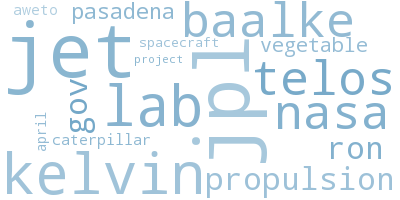
\includegraphics[width=0.14\columnwidth]{pics/Wordclouds/SpaceRelPrimp_2}
    &  
\includegraphics[width=0.14\columnwidth]{pics/Wordclouds/SpaceRelDBSSL_1}
    &  
\includegraphics[width=0.14\columnwidth]{pics/Wordclouds/SpaceRelDBSSL_2}
    \\
    & 
\includegraphics[width=0.14\columnwidth]{pics/Wordclouds/SpaceRelPunk_3}
    & 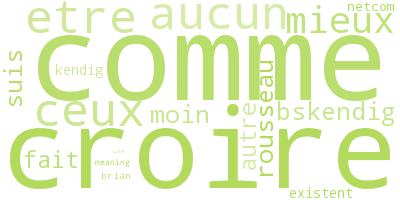
\includegraphics[width=0.14\columnwidth]{pics/Wordclouds/SpaceRelPunk_4}
    &  
\includegraphics[width=0.14\columnwidth]{pics/Wordclouds/SpaceRelPrimp_3}
    & 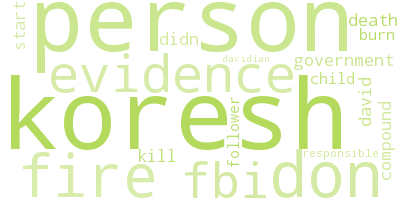
\includegraphics[width=0.14\columnwidth]{pics/Wordclouds/SpaceRelPrimp_4}
    &  
\includegraphics[width=0.14\columnwidth]{pics/Wordclouds/SpaceRelDBSSL_3}
    &  
\includegraphics[width=0.14\columnwidth]{pics/Wordclouds/SpaceRelDBSSL_4}
     \\\\
     \multirow{2}{*}{\rotatebox{90}{Politics}  }
    & 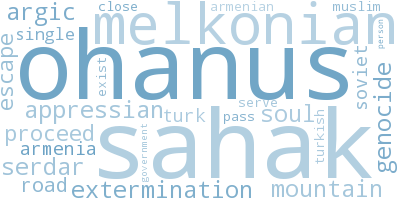
\includegraphics[width=0.14\columnwidth]{pics/Wordclouds/PolPunk_1}
    & 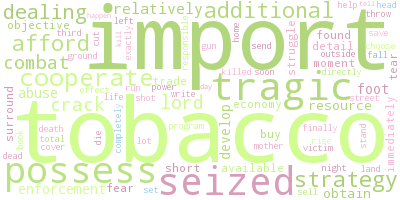
\includegraphics[width=0.14\columnwidth]{pics/Wordclouds/PolPunk_2}
    &  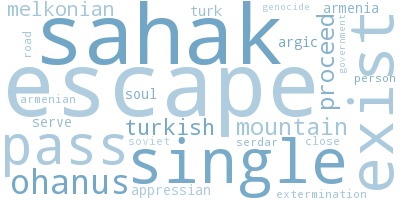
\includegraphics[width=0.14\columnwidth]{pics/Wordclouds/PolPrimp_1}
    & 
\includegraphics[width=0.14\columnwidth]{pics/Wordclouds/PolPrimp_2}
    &  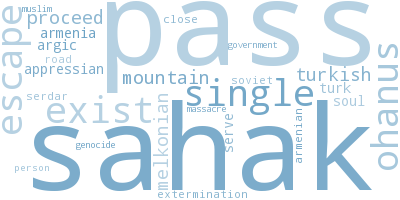
\includegraphics[width=0.14\columnwidth]{pics/Wordclouds/PolDBSSL_1}
    &  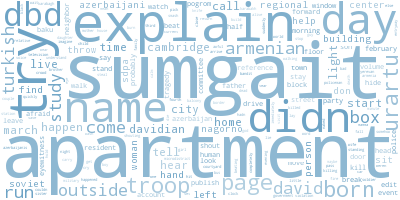
\includegraphics[width=0.14\columnwidth]{pics/Wordclouds/PolDBSSL_2}
    \\
    & 
\includegraphics[width=0.14\columnwidth]{pics/Wordclouds/PolPunk_3}
    & 
\includegraphics[width=0.14\columnwidth]{pics/Wordclouds/PolPunk_4}
    &  
\includegraphics[width=0.14\columnwidth]{pics/Wordclouds/PolPrimp_3}
    & 
\includegraphics[width=0.14\columnwidth]{pics/Wordclouds/PolPrimp_4}
    &  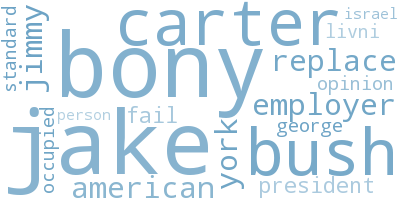
\includegraphics[width=0.14\columnwidth]{pics/Wordclouds/PolDBSSL_3}
    &  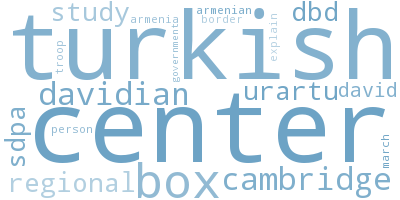
\includegraphics[width=0.14\columnwidth]{pics/Wordclouds/PolDBSSL_4}
     \\\\
    \multirow{2}{*}{\rotatebox{90}{Movie}  }
    & 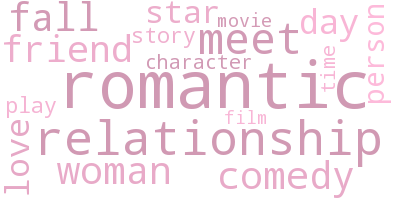
\includegraphics[width=0.14\columnwidth]{pics/Wordclouds/MoviePunk_4}
    & 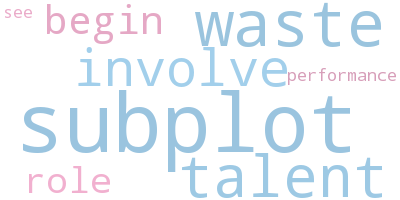
\includegraphics[width=0.14\columnwidth]{pics/Wordclouds/MoviePunk_1}
    &  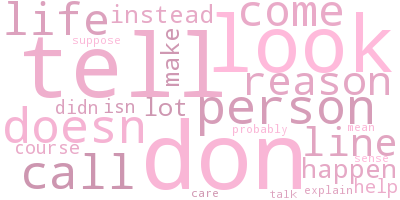
\includegraphics[width=0.14\columnwidth]{pics/Wordclouds/MoviePrimp_1}
    & 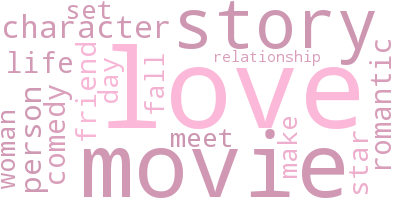
\includegraphics[width=0.14\columnwidth]{pics/Wordclouds/MoviePrimp_2}
    &  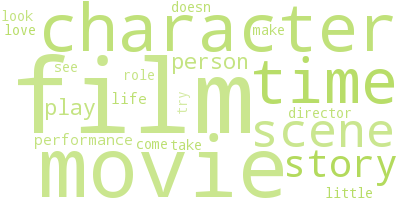
\includegraphics[width=0.14\columnwidth]{pics/Wordclouds/MovieDBSSL_1}
    &  
\includegraphics[width=0.14\columnwidth]{pics/Wordclouds/MovieDBSSL_2}
    \\
    & 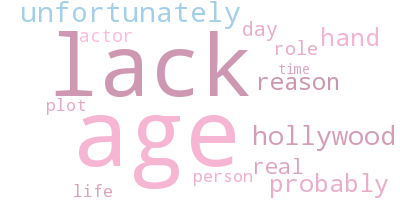
\includegraphics[width=0.14\columnwidth]{pics/Wordclouds/MoviePunk_2}
    & 
\includegraphics[width=0.14\columnwidth]{pics/Wordclouds/MoviePunk_3}
    &  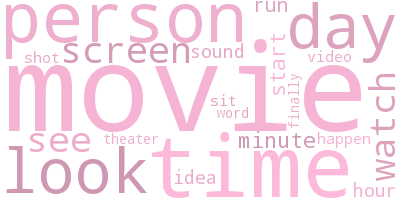
\includegraphics[width=0.14\columnwidth]{pics/Wordclouds/MoviePrimp_3}
    & 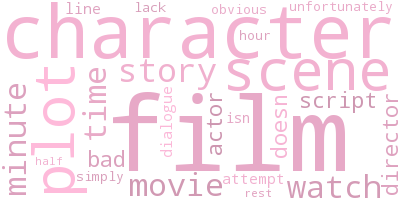
\includegraphics[width=0.14\columnwidth]{pics/Wordclouds/MoviePrimp_4}
    &  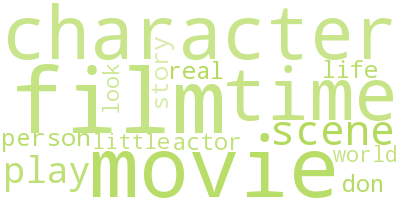
\includegraphics[width=0.14\columnwidth]{pics/Wordclouds/MovieDBSSL_3}
    &  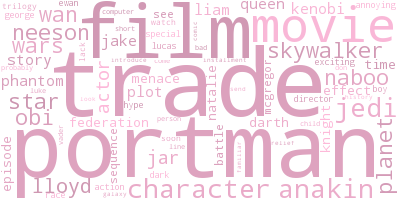
\includegraphics[width=0.14\columnwidth]{pics/Wordclouds/MovieDBSSL_4}
  \end{tabular}
  \caption{Illustration of a selection of derived topics for the 20 News and Movie datasets. The size of a word reflects its frequency in the topic ($\sim Y_{\cdot s}^\top D_{\cdot i}$) and the color its class affiliation: pink words are class-common, blue words belong to the first and green words to the second class. Best viewed in color.\label{fig:CS:topics}}
\end{figure}
Let us inspect the derived most prevalent topics in the form of word clouds.
Figure~\ref{fig:CS:topics} displays for every algorithm the top four topics, whose outer product (tile) spans the largest area. Class-common patterns are colored pink whereas class-specific patterns are blue or green. Class-specific alterations within topics become apparent by differently colored words in one word cloud. We observe that the topics displayed for the 20-Newsgroup data are mostly attributed to one of the classes. The topics are generally interpretable and even comparable among the algorithms (cf.\@ the first topic in the Politics dataset). Here, class-specific alterations of \textsc{C-Salt} point at the context in which a topic is discussed, e.g., the press release from the white house after a conference or meeting took place, whereby the latter may be discussed in both threads (cf.\@ the third topic for the Politics dataset).

The most remarkable contribution of class-specific alterations is given for the movie dataset. Generally, movie reviews addressing a particular genre, actors, etc., are not exclusively bad or good. \textsc{Primp} and \textsc{C-Salt} derive accordingly only common patterns. Here, \textsc{C-Salt} gives the decisive hint which additional words indicate the class membership. We recall from Table~\ref{tbl:CS:realWorld} that \textsc{DBSSL} returns in total four truncated topics for the Movie dataset. Thus, the displayed topics for the Movie dataset represent all the information we obtain from \textsc{DBSSL}. In addition, the topics display a high overlap in words, which underlines the reasonability of our assumption that minor deviations of common patterns denote for some datasets the sole class-distinctions.  
%=====================================
% Genome Data Analysis
%=====================================
\subsection{Genome Data Analysis}\label{sec:CS:gene}
The results depicted in the previous section are qualitatively easy to assess. We easily identify overlapping words and filter the important class characteristics from the topics at hand. 
In this experiment, the importance or meaning of features is unclear and researchers benefit from any summarizing information which is provided by the method, e.g., the common and class-specific parts of a pattern.
We regard the dataset introduced in~\cite{schramm2015mutational}, representing the genomic profile of 18 Neuroblastoma patients. For each patient, samples are taken from three classes: \emph{normal} (N), \emph{primary tumor} (T) and \emph{relapse tumor  cell} (R). The data denotes loci and alterations taking place with respect to a reference genome. Alterations denote nucleotide variations such as $A\rightarrow C$, insertions ($C\rightarrow AC$) and deletions ($AC\rightarrow A$). One sample from each of the classes N and T is given for every patient ($m_N=m_T=18$), one patient lacks one and another has three additional relapse samples ($m_R=20$), resulting in $m=56$ samples.   
We convert the alterations into binary features, each representing one alteration at one locus (position on a chromosome). The resulting matrix has $n\approx 3.7$ million columns.
\begin{figure}[!t]
\parbox[t]{.5\textwidth}{\null
  \centering
  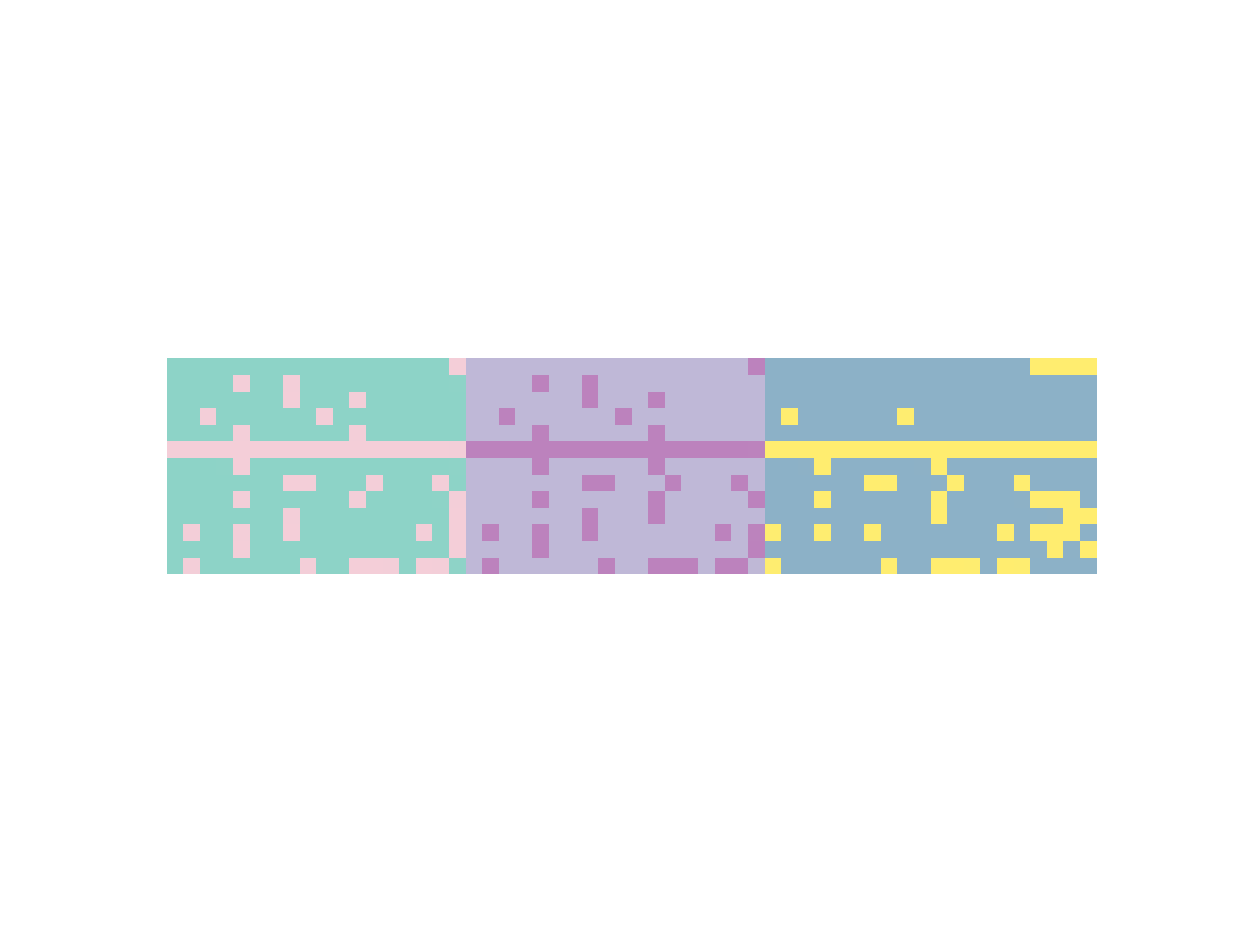
\includegraphics[trim={2.5cm 5.7cm  1cm 6.05cm},clip,scale=0.4]{pics/CSPatients.eps}%
  \captionof{figure}{Transposed usage matrix returned by \textsc{C-Salt} on the genome dataset. Class-memberships are signalized by colors.}\label{fig:GenY}%
}\qquad
\parbox[t]{.46\textwidth}{\null
\centering
  \vskip-\abovecaptionskip
  \captionof{table}[t]{Average size and empirical standard deviation of patterns $(\cdot 10^3)$ and class-specific alterations $(\cdot 10^3)$.}\label{tbl:genePatterns}%
  \vskip\abovecaptionskip
%   \begin{tabular}{cr} \toprule
%   $|V^{(N)}|$ & $2,066\pm 2,470$ \\ 
%   $|V^{(T)}|$ & $3,561\pm 4,776$ \\
%   $|V^{(R)}|$ & $3,784\pm 6,569$ \\ 
%   $|X|$ & $10,6797\pm 95,973$ \\\bottomrule
%   \end{tabular}
\setlength{\tabcolsep}{7pt}
\resizebox{.46\textwidth}{!}{%
  \begin{tabular}{rrrr} \toprule
  $|X|$ & $|V^{(N)}|$ & $|V^{(T)}|$ &  $|V^{(R)}|$ \\\midrule
  $10.7\pm 96$ & $2.1\pm 2.5$ 
   & $3.6\pm 4.8$ 
   & $3.8\pm 6.6$ 
	\\\bottomrule
  \end{tabular}
}
}
\end{figure}

\textsc{C-Salt} returns on the genome data a factorization of rank 32, of which we omit 20 patterns by means of the density bound (Theorem~\ref{thm:densProb}) with a noise assumption of $20\%$. Figure~\ref{fig:GenY} depicts the usage of the remaining twelve outer products, being almost identical for each class. Most notably, all derived patterns are class-common and describe the genetic background of patients instead of class characteristics. Table~\ref{tbl:genePatterns} summarizes the average length of patterns and corresponding class-specific alterations. We see that the average pattern reflects ten thousands of genomic alterations and that among the class-specific alterations, the ones which are attributed to relapse samples are highest in average. These results correspond to the evaluation in~\cite{schramm2015mutational}.

The information provided by \textsc{C-Salt} can not be extracted by existing methods. \textsc{Primp} yields only class-common patterns whose usage aligns with patients, regardless of classes. Running \textsc{Primp} separately on each class-related part $D^{(a)}$ yields factorizations of rank zero -- the genomic alignments between patients can not be differentiated from noise for such few samples.  
However, applying Vanilla \textsc{PAL-Tiling} separately, minimizing the RSS without any regularization for a specified rank of $15$, yields patterns for each part $D^{(a)}$. The separately mined patterns overlap over the classes in an intertwined fashion. The specific class characteristics are not easily perceived for such complex dependencies and would require further applications of algorithms which structure the information from the sets of vast amounts of features. This illustrates the importance of a global view on shared, discriminative and alterating patterns.
%======================
% Discussion
%======================
\section{Discussion}
We propose \textsc{C-Salt}, an explorative method to simultaneously derive similarities and differences among sets of transactions, originating from diverse classes. \textsc{C-Salt} solves a Boolean matrix factorization by means of numerical optimization, extending the method \textsc{Primp} to incorporate class assignments of the transactions. We integrate a factor matrix reflecting class-specific alterations of outer products from a BMF (cf.\@ Definition~\ref{def:CS:classSpecAlt}). Therewith, we capture class characteristics, which are lost by unsupervised factorization methods such as \textsc{Primp}. Synthetic experiments show that a planted structure corresponding to our model assumption is filtered by \textsc{C-Salt} (cf.\@ Figure~\ref{fig:CS:noise}). Even in the case of more than two classes, \textsc{C-Salt} filters complex dependencies among patterns and the classes (cf.\@ Figure~\ref{fig:synthClass}). These experiments also show that the rank is suitably estimated. On interpretable text data, \textsc{C-Salt} derives meaningful factorizations which provide valuable insight into prevalent topics and their class specific characteristics (cf.\@ Table~\ref{tbl:CS:realWorld} and Fig~\ref{fig:CS:topics}). An analysis of genomic data underlines the usefulness of our new factorization method, yielding information which none if the existing algorithms can provide (cf.\@ Section~\ref{sec:CS:gene}).
